%XXX Since design will focus on each component, this section can mirror the previous chapter, but instead of high level overview, describe how you implemented the description from the design chapter, programming language, libraries etc.

% Python
% Data collection - ccxt, binance, coinmarketcap
% historica data - anomaly detection - matplotlib -ohlcv - pandas - numpy 
% labeling - matplotlib - ohlcv - anomaly d
% generating dataset

\chapter{Implementation of \project}\label{ch:implementation}\glsresetall
This chapter describes the implementation of \project. It first, define the programming language and modules we use. Then it details how we implement each component.

We implement the system in the programming language \href{https://www.python.org/}{Python}, which is a powerful high-level scripting language that is excellent for building prototypes and conducting experiments. It has an extensive and superb standard library, in addition to an active community which provides specialized software that implements various protocols, \acp{api}, etc. It has roots in the following programming paradigms, procedural, object-oriented, and functional. In recent year, it has climbed to the very top of being the most popular programming language according to PYPL\footnote{Popularity of Programming Languge}~\cite{pypl_python}.

Python has an interpreter, a program that executes the code. Each python interpreter has a \ac{gil}, which is a mutex that protects access to the Python object, preventing multiple threads from executing Python bytecodes at once. This lock is necessary mainly because CPython's memory management is not thread-safe~\cite{python_gil}. Because of the \ac{gil}, a single interpreter cannot execute threads in parallel. To run parallel code in python, we must launch multiple interpreters. If we refer to a process, we refer process with its own interpreter, and we use a thread, then we refer to a thread that's running within an interpreter.

The modules we use are all available from PyPI\footnote{Python Package Index}, a python software repository, and they are all easily installable by using PyPI's package installer pip. The following modules we take advantage of are:

\begin{itemize}
    \item \textbf{ccxt} - package containing a uniform \ac{api} that implements numerous exchanges.
    \item \textbf{keras} - high-level deep learning network framework.
    \item \textbf{numpy} - fundamental scientific computing module.
    \item \textbf{pandas} - library containing data structures and data analysis tools.
    \item \textbf{matpotlib} - plotting library.
    \item \textbf{time-series} - module for working with time-series data.  
    \item \textbf{scikit-learn} - tools for data mining and analysis.
    \item \textbf{python-binance} - Python implementation of the exchange Binance.
    \item \textbf{CoinMarketCapAPI} - Python implementation of the cryptocurrency tracking site CoinMarketCap.
\end{itemize}

\section{Data Retriever}
%% MS
% Master
% Slaves - polymorphism
% Dataframe
We implement the data retriever as a master/slave architecture like described in \autoref{sec:master_slave}, where the master is a process, and the slaves are threads. So the master and the slaves are running inside a single interpreter. The slaves are assigned a source, and they will continuously pull data from the markets as long as they do not exceed their designated source request rate. Then, in a fixed interval, the master collects all the data from the slaves. All the slaves are different object instances, but they have the same \emph{interface}, allowing the master to exploit the concept of \emph{polymorphism} when retrieving the data from the slaves.

\begin{lstlisting}[language=python, caption={Data retriever's slave interface}, label=code:interface]
    class Slave(Thread):
        def __init__(self, markets):
        def header(self):
        def start(self):
        def stop(self):
        def row(self, market):
\end{lstlisting}

\autoref{code:interface} is the interface for each slave. The initializer method \texttt{\_\_init\_\_} initialize the internal state of each slave, and the argument is a list of markets that the slaves need to fetch data from. The \texttt{start} and \texttt{stop} will make the slave start and stopping retrieving market data, respectively. The \text{start} method starts a daemon that continuously retrieves data and caching it. The \texttt{header} returns a list of keys/names of the features it extracts from the markets, while \texttt{row}, returns the latest data from given market's cache, and parses it. Then, returns the features in a list in the same order as the keys/names. As long as the daemon run and fetch data, the cache will always contain the freshest data.

The execution flow of the data retriever, starts with the master initializes its slaves with markets they has to fetch data from. After the initialization, the master fetch each slave's list of headers in order to define the structure of the data, and have knowledge of the data retrieved from its slaves. All the headers is augmented and stored as the first row in a file that identifies a market, creating a data frame like \autoref{tab:dataframe}, where the headers are defined as $c$, and the data/feature is defined as $f$. Furthermore, the master and its slaves goes into a iterative phase, where in each iteration, the master retrieve the freshest data from its slaves. The data, then gets parsed such that each feature $f$ gets appended to their corresponding file and column $c$.
 
Naming the columns is convenient when having numerous features as it becomes easy to identify them. It will become practical when processing the data by indexing features by name, instead of indexing the features numerically, which is a hassle as we need a way to remember what each index means.

\begin{table}[ht]
    \centering
    \begin{tabular}{| r | r r r r |}
        \hline
                    & $c_1$     & $c_2$     & $\dots$   & $c_n$     \\
        \hline
        $1$         & $f_{1,1}$ & $f_{1,2}$ & $\dots$   & $f_{1,n}$ \\
        $2$         & $f_{2,1}$ & $f_{2,2}$ & $\dots$   & $f_{2,n}$ \\
        $\vdots$    & $\vdots$  & $\vdots$  & $\ddots$  & \vdots    \\
        $m$         & $f_{m,1}$ & $f_{m,2}$ & $\dots$   & $f_{m,n}$ \\
        \hline
    \end{tabular}
    \caption[Definition - Dataframe ]{A dataframe can be thought of as a dictionary-like container. Where the columns $c$, are names and represents keys, while the features $f$ are values that are mapped to a column.}
    \label{tab:dataframe}
\end{table}

\subsection{Sources}
We implement three slaves who are assigned different sources. The first slave is pulling data from the exchange Binance by using the module python-binance, the second is pulling data from multiple exchanges with the help of the module ccxt. Finally, the third slave pulls data from the cryptocurrency tracking site CoinMarketCap by using a module we create.

\subsubsection{Binance}
The exchange Binance provides various types of services through their \ac{api}. We only require the newest trading data regarding the markets given when initialized. We use their WebSocket \ac{api} that takes form as a \emph{pubsub} client where Binance pushes data to us. The first function that we subscribe on is the \emph{ticker} service, a $24$ hour rolling window containing statistics for a subscribed symbol that gets pushed every second~\cite{binance_git}. \autoref{code:binance_tick} shows the \ac{json} structure of the response of a ticker, and this response is returned for each market we subscribe on. In the ticker response, there are \ac{ohlcv} values for the past 24 hour and other additional features that may prove valuable when classifying \acp{pd}.

\begin{lstlisting}[language=json, caption={Ticker response from Binance (Source \cite{binance_git})}, label=code:binance_tick]
{
  "e": "24hrTicker",  // Event type
  "E": 123456789,     // Event time
  "s": "BNBBTC",      // Symbol
  "p": "0.0015",      // Price change
  "P": "250.00",      // Price change percent
  "w": "0.0018",      // Weighted average price
  "x": "0.0009",      // First trade(F)-1 price
  "c": "0.0025",      // Last price
  "Q": "10",          // Last quantity
  "b": "0.0024",      // Best bid price
  "B": "10",          // Best bid quantity
  "a": "0.0026",      // Best ask price
  "A": "100",         // Best ask quantity
  "o": "0.0010",      // Open price
  "h": "0.0025",      // High price
  "l": "0.0010",      // Low price
  "v": "10000",       // Base asset volume
  "q": "18",          // Quote asset volume
  "O": 0,             // Statistics open time
  "C": 86400000,      // Statistics close time
  "F": 0,             // First trade ID
  "L": 18150,         // Last trade Id
  "n": 18151          // Total number of trades
}
\end{lstlisting}

Furthermore, we also want the order book from Binance, who has proved to be valuable by two researchers at Standford as they were able to detect \ac{pd} with an accuracy of around $80\%$. So, in addition to subscribing on the ticker symbol, we also subscribe to Binance's \emph{depth} function. This function will return a response equal to \autoref{code:binance_depth}.

\begin{lstlisting}[language=json, caption={Depth response from Binance (Source \cite{binance_git})}, label=code:binance_depth]
{
  "lastUpdateId": 160,  // Last update ID
  "bids": [             // Bids
    [
      "0.0024",         // Price
      "10"              // Quantity
    ]
  ],
  "asks": [             // Asks
    [
      "0.0026",         // Price
      "100"             // Quantity
    ]
  ]
}
\end{lstlisting}

\subsubsection{ccxt}
The second slave uses the ccxt module, which provides a uniform \ac{api} access to various exchanges. We use this module to fetch \ac{ohlc} values over multiple exchanges. There are some complications with using this module because it provides uniform access to over $100$ exchanges, which becomes troublesome when the slave is initiated with the markets it has to fetch data from, and we do not have any prior knowledge of the exchanges markets.

So, we first create a reverse map, where we map markets to a list of exchanges. This is done by initiating all the exchanges from the ccxt module and request all the exchanges' markets and map each market to a list of exchanges. Then, we define \ac{pubsub} that \autoref{fig:ccxt} illustrates. Where the exchanges are the publishers and fetch market data and propagate it to the broker. Subscribers issue interest in a specific market to the broker. The broker synchronizes the exchanges and makes sure them issues request simultaneously, and when all the exchanges have returned propagated their response, it aggregates all the data from each coin. Finally, the broker pushes the data to the subscribers using a callback function which was given when the subscribers first issued their interest.

\begin{figure}
    \centering
    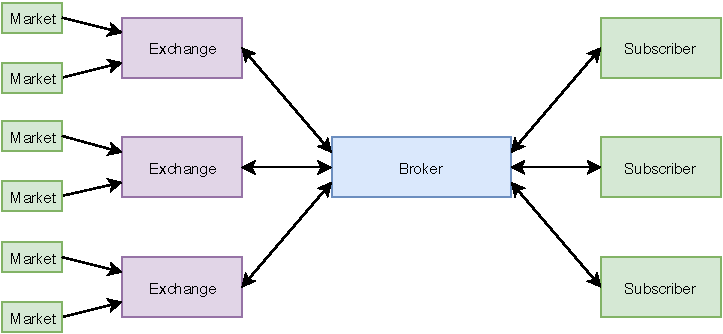
\includegraphics[width=\textwidth]{marketpull.pdf}
    \caption[\project's Publish/Subscribe system]{overview of fetching data from multiple sources.}
    \label{fig:ccxt}
\end{figure}

The method we use to extract market data from ccxt's uniform \ac{api} is the ticker function, which contains more or less the same information given by Binance, but the information we use is only the \ac{ohlc} values. With the reverse map we create, we can also estimate the ratio of how many exchanges that lists a specific market as this feature was explicitly described in \autoref{tab:pd_characteristics} as a characteristic of a \ac{pd}.

\subsubsection{CoinMarketCap}
The final slave retrieves data from \href{https://coinmarketcap.com/}{CoinMarketCap}, which is a popular cryptocurrency tracking site and contains statistics regarding a coin's capitalization, circulation, etc. We have to use CoinMarketCap private \ac{api} as they recently deprecated their public \ac{api}. Using their private \ac{api} is intuitive, the identification is an \ac{api} key, but CoinMarketCap has defined a severe complex request system. Where a user has a load of credits, and the amount of credit one has, depends on the type of subscription one has . A user also has a daily, weekly, and monthly request rate system, which also depends on the type of subscription on have. There are some Python modules in existence that allows one to extract data from CoinMarketCap, but they completely ignore the request system, which, when used will be problematic as we continuously will exceed the request limit and credit system, which ultimately results in a permanent ban from using their \ac{api}.

Thus, we create a module that supports throttling of requests, which adjusts to both the credit system and the number of requests one can issue. We cache every request in an SQLite database because CoinMarketCap mostly provides data that rarely or slightly change. The cache also comes with an exceed factor allowing one to adjust when cached data shall be removed from the cache. There are four endpoints in CoinMarketCap, where each endpoint has a set of functions:

\begin{itemize}
    \item Cryptocurrency
    \item Exchanges
    \item Globals
    \item Tools
\end{itemize}

We use the modules requests, requests\_cache, and ratelimit. We use the requests module for making requests to CoinMarketCap's \ac{api}. Requests\_cache is monkey patch to the request module, and caches every request made by it. The ratelimit allows to define function decorators that restricts the number of function calls within an interval.

The module fetches data from the cryptocurrency endpoints. The majority of the functions in CoinMarketCap requires a paid subscription, but we are only using two free functions. The first function returns the global metrics, which contains total market capitalization. The second function lists cryptocurrencies' latest market data that contains fields like circulation supply for each market, and it defines the total amount a cryptocurrency is worth. CoinMarketCap does provide market data, but since we cache every request and the request limit is limited to $333$ requests a day, we can not use it as it results in us using stale data.


\section{Data Preparing}
After gathering enough data, we can start to prepare it for \ac{ml}. Each market has a file containing data from the sources we recently described. Since we prepare the data in the files equally, we can speed up the operations by processing the files in parallel. Each file we have to process can be small in general, but combining them all, they may become quite large. Hence, we only process a fixed number of files in parallel.

We parallelize every operation by creating, yet again, a master/slave structure where the master process spawns the same number of child processes (slaves) as there are markets. The slaves are initialized with a market, a semaphore to control the number of processes to run inside a critical section, and a queue to signalize to the master when it's done. Inside the critical section, the child loads the dataset, and execute the desired operation accordingly and stores the results. After the child leaves the critical section, it signalize back to the master.  The slaves use the module Pandas to load each dataset into a date frame. With a data frame, a slave is able to index features by their column name, which makes it convenient when we do cleansing and feature engineering. 

The first number of operations involves cleansing the data. We cleanse by removing corrupted files. We also remove the features that are not needed, e.g, in \autoref{code:binance_tick}, the constant categorical field \texttt{symbol} are not needed when classifying \ac{pd}. The last cleansing process we do is to interpolate the data. Values involving price and quantity gets linearly interpolated as we describe in \autoref{ch:design}.

The second series of operation we do is creating new features. We calculate the percentage of change like described in \autoref{ch:design} on all the values we interpolated. Then we create new features from using the timestamp that we added along with the data when it was stored. Finally, we create a new feature that describe the imbalance of the order book.

\section{Collecting pump-and-dumps}
We use the anomaly detection algorithm to detect \acp{pd}, which we described in \autoref{ch:design}. It marks an interval anomalous if there is a significant increase in price and volume in that period compared to the previous periods. We do not use the anomaly detection algorithm with the data that was collected in real-time, as this data is not compliant with the algorithm. Instead, we retrieve historical \ac{ohlc} data from Binance that span over the period we gathered data.

The algorithm uses sliding a window containing a fixed number of \ac{ohlcv} values. We create a sliding window module which is wraps around a python list. With the sliding window, it becomes easy to initialize a fixed size list, and when adding new elements to the list, the last element will be removed, just like a fixed size \ac{fifo} structure.

\autoref{code:binance_kline} illustrates a response from Binance that contains historical \ac{ohlc} values. With these values and a sliding window, we start to continuously add \ac{ohlcv} values that span over the period we collected data, as we iteratively calculate whether the newest added \ac{ohlc} is an anomaly compared to the other \ac{ohlc} values in the window. The fields we use from \autoref{code:binance_kline} are \texttt{close} and \texttt{high} when calculating whether the price surpasses a specified price threshold, while we use the field \texttt{volume} when calculating whether volume exceeds a specified volume threshold.

\begin{lstlisting}[language=json, caption={Historical kline response from Binance (Source \cite{binance_git})}, label=code:binance_kline]
[
  [
    1499040000000,      // Open time
    "0.01634790",       // Open
    "0.80000000",       // High
    "0.01575800",       // Low
    "0.01577100",       // Close
    "148976.11427815",  // Volume
    1499644799999,      // Close time
    "2434.19055334",    // Quote asset volume
    308,                // Number of trades
    "1756.87402397",    // Taker base volume
    "28.46694368",      // Taker quote volume
  ]
]
\end{lstlisting}

As we have previously mentioned,  anomaly detection algorithms tend to have a high occurrence of false positive compared to true positive. So we remove the false positives by first plotting finer-grained \acp{ohlc} values over the periods that were flagged anomalous in each market. Then, removing the anomalies that we believe is not a \ac{pd}, while retaining the anomalies that we believe is a \ac{pd}. We plot the \ac{ohlc} values by using the matplotlib module in Python.

After filtering \acp{pd}, we can label the features that we have created. We use the same master/slave method, which we used during the feature engineering stage. Where each process is initiated with a semaphore and queue, but also the \ac{pd} anomalies. To label the dataset, slaves loads its assigned dataset and identify the interval where the \ac{pd} occurred, and find the points where the most significant change in price percent happened. From the highest point, we label the points as positive from where the change in percent was positive until it becomes negative.

\section{Deep Learning}
Before we can train the model, we normalize each market using the min-max method described in \autoref{ch:design}. We have to process the data over two iterations, in the first iteration, we iterate over all the markets to find the greatest and smallest value in the features. Then, in the second iteration, we normalize the features.

To create a balanced dataset, we undersample the data. So, we first have to collect all the positive samples from the datasets. Then we select random negative sequences from them until the number of negative and positive samples are approximately equal.

We use the deep learning library Keras for building the model, and the first layer contains \ac{lstm} cells and the second layer contains a single perceptron. Training a \acp{lstm} network requires us to reshape our 2D input data, into a 3D shaped matrix. The 3D shape represents matrices inside a matrix. A sample in a 3D space is a matrix containing a batch of vectors within a time lag. Then the third dimensions is a batch of these new samples. After shaping our data, we can finally train our model.
